\documentclass[journal,letterpaper]{IEEEtran}

\usepackage{cite}
\usepackage{graphicx}
\usepackage{amsmath,amssymb}
\usepackage{algorithm}
\usepackage{algorithmic}
\usepackage{psfrag}

\IEEEoverridecommandlockouts

% AML bibliography references
\newcommand{\bib}[1]{/aml/home/mjg82/bib/#1}

% Better references, I think
\renewcommand{\sec}[1]{Section~\ref{sec:#1}}
\newcommand{\fig}[1]{Figure~\ref{fig:#1}}
\newcommand{\alg}[1]{Algorithm~\ref{alg:#1}}

% Algorithmic changes
\renewcommand{\algorithmicforall}{\textbf{for each}}

%% PSO Stuff
\DeclareMathOperator*{\argmin}{arg\;min}
\DeclareMathOperator*{\argmax}{arg\;max}
\DeclareMathOperator*{\arginf}{arg\;inf}
\DeclareMathOperator*{\argsup}{arg\;sup}
\providecommand{\pers}{\ensuremath{P}}
\providecommand{\neigh}{\ensuremath{N}}
\providecommand{\leftind}{\ensuremath{L}}
\providecommand{\rightind}{\ensuremath{R}}
\providecommand{\nURand}{\ensuremath{U^\neigh}}
\providecommand{\pURand}{\ensuremath{U^\pers}}
\providecommand{\ppos}{\ensuremath{\Vec{x}}}
\providecommand{\fppos}{\ensuremath{\Vec{fx}}}
\providecommand{\pvel}{\ensuremath{\Vec{v}}}
\providecommand{\nbest}{\ensuremath{\Vec{b}^\neigh}}
\providecommand{\fnbest}{\ensuremath{\Vec{fb}^\neigh}}
\providecommand{\pbest}{\ensuremath{\Vec{b}^\pers}}
\providecommand{\fpbest}{\ensuremath{\Vec{fb}^\pers}}
\providecommand{\constriction}{\ensuremath{\chi}}
\providecommand{\ncoeff}{\ensuremath{\phi^\neigh}}
\providecommand{\pcoeff}{\ensuremath{\phi^\pers}}
\providecommand{\obs}{\ensuremath{\Vec{\xi}}}
\providecommand{\ofunc}{\ensuremath{f}}
\providecommand{\swarm}{\ensuremath{swarm}}

%SpecExPSO Stuff
\providecommand{\indic}{\ensuremath{I}}
\providecommand{\specvel}{\ensuremath{\vec{V}}}
\providecommand{\specpos}{\ensuremath{\vec{X}}}
\providecommand{\leftn}{\ensuremath{\Vec{x}^\leftind}}
\providecommand{\rightn}{\ensuremath{\Vec{x}^\rightind}}
\providecommand{\caseset}{\ensuremath{\mathcal{C}}}
\providecommand{\casedef}{\ensuremath{(\pbest,\nbest)}}
\providecommand{\casexn}{\ensuremath{(x,\neigh)}}
\providecommand{\casexx}{\ensuremath{(x,x)}}
\providecommand{\casexl}{\ensuremath{(x,\leftind)}}
\providecommand{\casexr}{\ensuremath{(x,\rightind)}}
\providecommand{\casepn}{\ensuremath{(\pers,\neigh)}}
\providecommand{\casepl}{\ensuremath{(\pers,\leftind)}}
\providecommand{\casepr}{\ensuremath{(\pers,\rightind)}}
\providecommand{\noeval}[1]{\ensuremath{#1^{-e}}}
\providecommand{\nonbest}[1]{\ensuremath{#1^{-n}}}
\providecommand{\p}{\ensuremath{p}}
\providecommand{\pset}{\ensuremath{\mathbf{p}}}
\providecommand{\s}{\ensuremath{s}}
\providecommand{\sset}{\ensuremath{\mathbf{s}}}
\providecommand{\nsset}{\ensuremath{\mathbf{ns}}}
\providecommand{\n}{\ensuremath{n}}
\providecommand{\nset}{\ensuremath{\mathbf{n}}}
\providecommand{\nnset}{\ensuremath{\mathbf{nn}}}

%Other math
\providecommand{\prob}{\ensuremath{\mathrm{Pr}}}

\title{\ \\ \LARGE\bf Speculative Evaluation in Particle Swarm Optimization%
\thanks{Matthew Gardner, Andrew McNabb, and Kevin Seppi are with the Department
of Computer Science, Brigham Young University, 3361 TMCB, Provo, UT 84602
(phone: 801-422-8717; email: \{mjg82,a,k\}@cs.byu.edu).}%
}

\date{}

\author{Matthew Gardner, Andrew McNabb, and Kevin Seppi}

\begin{document}
\maketitle

\begin{abstract}

Particle swarm optimization (PSO) has previously been parallelized only by 
adding more particles to the swarm or by parallelizing the evaluation of the
objective function.  However, in many cases this approach does not scale to 
very large populations sizes (on very large clusters).
In response to this issue, we take inspiration from 
speculative execution commonly performed in modern processors and propose
Speculative Evaluation in PSO (SEPSO).

In SEPSO future positions of the particles are
speculated and evaluated in parallel with the evaluation of current positions.
We show that the set of speculative evaluations will always include the position and corresponding
evaluation that would normally have occurred at the next iteration.
Thus SEPSO performs two
iterations of PSO at once, allowing it to achieve better fitness faster.
Not only can SEPSO can achieve better fitness in the same number of iterations,
it also reaches better fitness for the same number of total function evaluations
in large scale parallel environments.

While Speculative Evaluation in PSO is an intriguing idea, its
usefulness is limited unless some slight modifications are made to the PSO
algorithm.  By relaxing the requirement that speculative evaluation exactly
reproduce the behavior of the original PSO, we can make better use of the information
obtained by the speculative evaluations.
Using these algorithmic modifications, we see dramatic improvements in the
effectiveness of the algorithm. 
\end{abstract}

\section{Introduction}
\label{sec:intro}

Particle swarm optimization (PSO) has been found to be a highly robust and
effective algorithm for solving many types of optimization problems.  For much
of the algorithm's history, PSO was run serially on a single machine.  However,
the world's computing power is increasingly coming from large clusters of
processors.
%Even in desktop machines, systems with 4 or 8 cores are
%commonplace.  
In order to efficiently utilize these resources for
computationally intensive problems, PSO needs to run in parallel.

Within the last few years, researchers have begun to recognize the need to
develop parallel implementations of PSO, publishing many papers on the subject.
The methods they have used include various synchronous algorithms
\cite{mcnabb-cec07,belal-ijicis04,chu-sci06,jin-aps05,parsopoulos-aia04,schutte-ijnme04},
and asynchronous algorithms \cite{koh-ijnme06,mostaghim-report06,venter-wcsmo05}.
Parallelizing the evaluation of the objective function can also be done in some
cases, though that is not an adaption of the PSO algorithm itself and thus is
not the focus of this paper.

These previous parallel techniques use additional processors to increase the
number of particles in the swarm, either by adding individual particles or by
adding entire new sub-swarms but in all cases
the number of processors never exceeds the number of particles.
The number of iterations of PSO that the
algorithms can perform is thus inherently limited by the time it takes to
evaluate the objective function---additional processors add more particles, not
more iterations.

The purpose of this paper is to consider pso parallelization strategies for
clusters of thousands of processors and functions for which a single
evaluation will take at least minutes, but probably hours or perhaps days.
Our purpose is to explore the question ``Since pso is often run with
a swarm of size of 50-100, what would one do if a few thousand processors were available?''

For many functions there comes a point of diminishing returns with respect to adding particles.
In \fig{basic-sphere} we show the value obtained after 20,000 function evaluations (not iterations)
as a function of swarm size
for the well-know benchmark function Sphere (20 dimensions, reporting the average of thirty runs). 
Increasing the swarm size from 10 to 50 has a significant effect value obtained
however, increasing the swarm size from 100 to 200 makes the algorithm less efficient,
reducing the progress the algorithm makes per-evaluation.
For this reason, research recommends the use a swarm size of 50 for this function
~\cite{bratton-sis07}.
Thus, in at least some cases, added particles indefinitely will not yield an efficient implementation. 

\begin{figure}
  \centering
  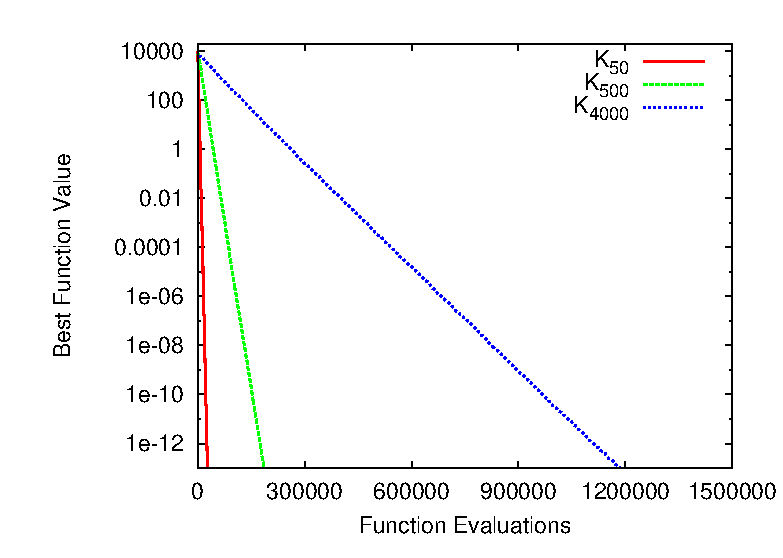
\includegraphics[width=.8\columnwidth]{evals_sphere.eps}
  \caption{Function Sphere with a swarm with various swarm sizes.}
  \label{fig:evals-sphere}
\end{figure}

To solve this problem, we take inspiration from speculative execution
techniques commonly used in processors.  Modern processors, when faced with a
branch on which they must wait (e.g. a memory cache miss), guess which way the
branch will go and start executing.  If the processor guesses right, execution
is much farther ahead than if it had just idly waited on the branch.  If it
guesses wrong, execution restarts where it would have been anyway.
This is called speculative execution or branch prediction.

The idea of speculative execution can be applied to some types of optimization
algorithms.  When the next sampling position of the algorithm does not depend
on the value of the objective function at the current position,
future positions can be speculated and evaluated in parallel with the current
position.
This is trivially true for optimization by random sampling, for example.
The next random sample does not depend on the previous point nor on the value
of the objective function at that point in any way.
It depends only on a random number.
There is no need to wait to see
what objective function value was obtained at the previous point,
evaluation of the object function at the next point can begin as soon as the next random number is drawn.
In other optimization algorithms, the next position depends on the previous position, but not the
value obtained there, a random walk for example.
In this case
the next position to be evaluated
depends only on the previous position and a random number.
In this case, as it was in the case of random sampling,
the object function evaluation of the next position can be done in parallel
because it 
does not depend on the \emph{value} of the objective function at the previous position.
There are an infinite number of possible next positions, but only one given the draw of the random number.

In still other cases, the next position to be evaluated may depend on the current position and some
discrete valued (binary, for example) test on the value obtained at the previous position. In such
cases all of the next possible positions can be evaluated at the same time as the
evaluation of the current position.
One of these speculative positions will exactly preserve the behavior of the algorithm
and the others are wasted.
This approach has been applied to 
simulated annealing where the next position depends on (1) the last position, (2) a random number
and (3) the result of a binary test comparing the value of the objective function at the current state with the value of the objective function at the
last position.
In this context the next position can be computed in the case where the binary test is true
and in the case where it is false.
in simulated annealing to compute (1) the value of the objective function at the current position,
(2) the value at the position if the test turns out to be true and (3) the value at the position
if the test turns out to be false; all in parallel.
The test can be evaluated once all three of these evaluations of the objective function are complete, thus
computing all of the objective function evaluations
needed for two iterations in parallel and all at once~\cite{witte-tpds91}.
For all but the most computationally-trivial objective functions, this approach saves almost half of the
``wall-clock'' time.
By way of contrast, this approach can not be used in gradient methods where the
step size for sampling typically depends on the gradient and therefor the position and \emph{value}
at the current position. In this case there are an infinite number of possible speculative
evaluations.

% Use this later?
% Skip this??
% 
% Speculative evaluation is possible in PSO because the motion of particles
% depends only on the \emph{positions} of the particle and its best neighbor, not
% the \emph{value} of the objective function at those positions.  We do not have
% to wait for a particle's function evaluation to complete in order to know where
% it might move to next, so we can compute the set of all possible next positions
% and send them to be evaluated along with the particle's current position.  Once
% the current position of each particle has been evaluated, we can determine
% which of the speculatively evaluated positions matches the branch taken by the
% particle.  We have thus evaluated two iterations at once.  This can easily get
% unwieldy if the set of next possible positions for each particle is large, but
% a wise choice of topology limits that set to a reasonable size.
% 
% But the following does need some intro

In this paper we show that the results of standard PSO can be reproduced \emph{exactly}, two iterations at a time, using
a speculative evaluation approach like the ones described above. We prove that this approach
produces exactly equivalent results, and demonstrate this by implementation.
The resulting implementation runs efficiently on large clusters where the number of processors is much larger than
a typical or reasonable number of particles. Producing better results in less ``wall-clock'' time and,
surprisingly, with fewer total function evaluations.

Furthermore, we show that if we relax the requirements of the algorithm, no
longer demanding that it strictly reproduce the exact behavior of standard PSO, we
can introduce new speculative techniques that often out-perform PSO.
These variants make better use of the extra information obtained from
the extra exploration made by the speculative function evaluations.
We also explore the idea that, like branch prediction in processors, we
need not speculatively evaluate \emph{all} possible future positions,
We can accelerate the algorithm even if we are just \emph{likely} to have guessed right.
By pruning the speculation to just paths that are statistically likely to reproduce pso we can also 
speculating several iterations ahead instead of just one.
We also consider several recovery strategies for cases where
the pruned set of speculative evaluations does not contain the evaluation that standard pso would have done.

The balance of this paper is organized as follows:
\sec{pso} describes the particle swarm optimization algorithm.
\sec{sepso}
describes how speculative evaluation can be done in parallel PSO to
perform two iterations at once, then presents a comparison of the speculative
algorithm with the original PSO.  In \sec{relax}, we discuss various methods of
improving the performance of speculative evaluation in PSO, all of which break
the requirement of strictly reproducing the behavior of the original algorithm.
In \sec{conclusion} and \sec{future} we conclude and discuss future work.

\section{Particle Swarm Optimization}
\label{sec:pso}

Particle swarm optimization was proposed in 1995 by James Kennedy and Russell
Eberhart~\cite{kennedy-icnn95}.  The algorithm is used to intelligently search
a multi-dimensional space by mimicking the swarming and flocking behavior of
birds and other animals. It is a social algorithm that depends on interaction
between particles to quickly and consistently approximate the optimal solution to a
given objective function.

The motion of particles through the search space has three components: an
inertial component that gives particles momentum as they move, a cognitive
component where particles remember the best solution they have found and are
attracted back to that place, and a social component by which particles are
attracted to the best solution that any of their neighbors have found.

At each iteration ($t+1$) of the algorithm, the position $\ppos_t$ and velocity
$\pvel_t$ of each particle are updated as follows:
\begin{align}
\nonumber
	\pvel_{t+1} &=
		\constriction \bigl[ \pvel_t
			+ \pcoeff\pURand_{t}\otimes(\pbest_{t} - \ppos_{t}) \\
\label{eq:velupdate}
			& \quad \quad \quad \, + \ncoeff\nURand_{t}\otimes(\nbest_{t} - \ppos_{t})
		\bigr] \\
\label{eq:posupdate}
	\ppos_{t+1} &= \ppos_{t} + \pvel_{t+1}
\end{align}
where \( \nURand_{t} \) and \( \nURand_{t} \) are vectors of independent
and identically distributed random numbers drawn from a uniform
distribution, the \( \otimes \) operator is an element-wise vector
multiplication, $\pbest$ (called personal best) is the best position the
current particle has seen, and $\nbest$ (called neighborhood best) is the best
position the neighbors of the current particle have seen~\cite{bratton-sis07}.  \( \ncoeff \), \(
\pcoeff \), and \( \constriction \) are parameters with prescribed values
required to ensure convergence (2.05, 2.05, and .73,
respectively)~\cite{clerc-tec02}. Note also that we use a subscript for the 
time step $t$ or $t+1$ and have moved all other qualifiers,
such as the personal $\pers$ qualifier to the superscript position.
Superscripts can be miss read as exponents, but they are qualifiers throughout this paper.

There are many ways of defining the neighbors of a particle. 
Changing the
neighborhood topology has a significant effect on the performance of the algorithm and 
this effect varies widely by function type, as would be expected by the No Free Lunch
theorem~\cite{wolpert-tec97}.
The two most common topologies used in the
literature are the Ring topology and the Complete
topology~\cite{bratton-sis07}.  In the Ring topology, each particle has one
neighbor to either side of it; in the Complete topology, every particle is a
neighbor to every other particle.  In all topologies, a particle is also a
neighbor to itself, in that its own position is considered when updating the
particle's $\nbest$.  Thus with $p$ particles, using the Ring topology each
particle has three neighbors: $i-1$, $i$ (itself), and $i+1$.  With the Complete
topology, each particle has $p$ neighbors.
% TOD USE THIS LATER!
% In this paper we use these
% topologies, as well as a parallel adaptation of the Complete topology, called
% Random, that has been shown to simulate the behavior of Complete with far less
% communication~\cite{mcnabb-cec09}.  In the Random topology, each particle
% randomly picks two other particles to share information with at each iteration,
% along with itself.  Thus in both the Ring and the Random topologies, all
% particles have 3 neighbors.

\section{Speculative Evaluation in PSO}
\label{sec:sepso}
\subsection{Overview}

The PSO algorithm can be trivially parallelized by distributing the processing needed for each
particle on a separate processor.
But as we have seen in the introduction, for some
functions, and for large numbers of processors where just adding particles (processors)
reaches a point of diminishing returns.
That is, adding processors does not help us reach any given level of fitness appreciably faster.

To address this issue we present here a very different use of additional processors.
Performing more iterations instead of adding more particles (for a fixed number of function evaluations),
previous techniques have not addressed this issue.
In order to perform additional iterations by adding additional processors, we
take inspiration from speculative execution in processors.
We do this by refactoring the standard PSO equations as described here.

%First consider formula for the \emph{next} iteration of PSO, which is identical
%to Equations~\eqref{eq:velupdate} and \eqref{eq:posupdate} except the time
%subscripts are incremented.  As noted above and
For simplicity in this
explanation, we restrict our discussion here to the case of a Ring topology
with two neighbors which we will call the ``right neighbor'' and ``left
neighbor'' neighbors identified for each particle as $\rightn$ and $\leftn$
respectively.

Next note that the computation of $\pbest$ and $\nbest$ is not seen in the
update equations~\eqref{eq:velupdate} and \eqref{eq:posupdate}, so we will make
this mathematically explicit.  This update is usually implemented as a pair of
independent ``if``-statements, but that is a bit awkward for our purposes
so we instead use a set of indicator variables, one each representing each
possible update to the \emph{pair} $\casedef$.  These indicator variables allow
us to easily identify the cases in which updates will be needed for $\nbest$,
$\pbest$ or both.

For example, we can write $\casexn$ to identify the case where $\pbest$ will be
updated with the better position $\ppos_{i,t}$, shown in the first positions,
but a no new neighborhood best was found so $\nbest$ remains in the second
position.

For any topology with 2 neighbors there are 7 possible update cases listed in
Table~\ref{tab:evals}.  This list assumes, as is typically the case, that each
particle is also part of its own neighborhood (can cause an update to
$\nbest$). The list also omits the case where $\nbest$ is updated by
$\ppos_{t}$ but $\pbest$ was not updated, as this is logically impossible.
$\caseset$ represents the set of all cases.

For minimization, we can define this example indicator variable representing the case
where the particle will need to update $\pbest$ with the better
position $x_{t}$ for the next iteration ($t+1$), but $\nbest$ will not updated by:
\begin{align}
\nonumber
	\indic_{t+1}^{\casexn} & (\ofunc ( \ppos_{t+1} ) ,\ofunc(\leftn_{t+1}),\ofunc(\rightn_{t+1}) ,\ofunc(\pbest_{t}) ,\ofunc(\nbest_{t}))= \\
\nonumber
	& 1 \ if \  \ofunc(\ppos_{t+1}) > \ofunc(\pbest_{t}) \\
\nonumber
	& \quad \quad \ \wedge \ \ofunc(\nbest_{t}) > \ofunc(\ppos_{t+1}) \\
\nonumber
	& \quad \quad \ \wedge \ \ofunc(\nbest_{t}) > \ofunc(\leftn_{t+1}) \\
\nonumber
	& \quad \quad \ \wedge \ \ofunc(\nbest_{t}) > \ofunc(\rightn_{t+1}) \\
\label{eq:deficasexn}
	& 0 \ otherwise
\end{align}

For compactness in our equations we represent this without the parameters since
they can be inferred from the subscripts on $\indic_{t}^{\casexn}$.  The
indicator variables for the other update cases shown in Table~\ref{tab:evals}
($\casepn$, $\casepl$, $\casepr$, etc.) can be defined in similar fashion but
obviously using the corresponding boolean expression.

For each cases identified in Table~\ref{tab:evals} and identified by a
corresponding indicator variable defined above, we also provide notation for the \emph{next} velocity
update equation; once again using $\casexn$ as an example:
\begin{align}
\nonumber
	\specvel_{t+1}^{\casexn} & (\pvel_t, \ppos_{t+1}, \leftn_{t+1}, \rightn_{t+1}, \pbest_{t},
        \nbest_{t}, \pURand_{t}, \nURand_{t}) \\
\label{eq:defvocasexn}
		&= \constriction \bigl[ \pvel_{t} +
			\pcoeff\pURand_{t+1}\otimes(\pbest_{t+1} - \ppos_{t+1}) \\
		& \quad \quad \quad \; + \ncoeff\nURand_{t+1}\otimes(\nbest_{t+1} - \ppos_{t+1})
		\bigr]
\end{align}

Again we will drop the parameters for compactness and since
they can be inferred from the subscripts on $\specvel_{t}^{\casexn}$.
The update equation is taken exactly from the standard update equations~\eqref{eq:velupdate}
and \eqref{eq:posupdate}, but
since it is restricted to a specific case, $\casexn$ for this example,
it is no longer necessary to use $\pbest$ and $\nbest$, since in this case
$\pbest_{t+1}=\ppos_{t+1}$ and $\nbest_{t+1}=\nbest_{t+1}$ we can re-write
$\specvel_{t+1}^{\casexn}$ as:
\begin{align}
\nonumber
	\specvel_{t+1}^{\casexn} &= \constriction \bigl[ \pvel_{t} +
			\pcoeff\pURand_{t+1}\otimes(\ppos_{t+1} - \ppos_{t+1}) \\
\label{eq:defvcasexn}
			& \quad \quad \quad \; + \ncoeff\nURand_{t+1}\otimes(\nbest_{t+1} - \ppos_{t+1})
		\bigr]
\end{align}

For each cases identified in
Table~\ref{tab:evals}
and identified by a corresponding indicator variable defined above,
we define also a position update equation with its compact form; once again using $\casexn$ as an example:
\begin{align}
\label{eq:defpcasexn}
	\specpos_{t+1}^{\casexn} & (\ppos_{t}, \pvel_{t},\ppos_{t+1} ,\leftn_{t+1},\rightn_{t+1} ,\pbest_{t} ,\nbest_{t})= \\
\nonumber
	& = \specpos_{t+1}^{\casexn} =  \ppos_{t} + \specvel_{t+1}^{\casexn}
\end{align}

Lastly, we use the normal notation for the value of the objective function at these points,
once again using the case $\casexn$ as an example:
\begin{align}
\nonumber
	\ofunc(\specpos_{t+1}^{\casexn} & (\ppos_{t+1} ,\leftn_{t+1},\rightn_{t+1} ,\pbest_{t} ,\nbest_{t}))= \\
\label{eq:deffcasexn}
	& =  \ofunc(\specpos_{t+1}^{\casexn})
\end{align}

With this notation we can re-write the ``next iteration'' form of the original PSO motion equations
given in equations~\eqref{eq:velupdate}
and \eqref{eq:posupdate} as:
\begin{align}
\nonumber
	\pvel_{t+1} &=
		\constriction \bigl[ \pvel_t
			+ \pcoeff\pURand_{t}\otimes(\pbest_{t} - \ppos_{t}) \\
\nonumber
			& \quad \quad \quad \, + \ncoeff\nURand_{t}\otimes(\nbest_{t} - \ppos_{t})
		\bigr] \\
\nonumber
	&= \sum_{c \in \caseset} \constriction \bigl[ \pvel_t
			+ \pcoeff\pURand_{t}\otimes(\pbest_{t} - \ppos_{t}) \\
\nonumber
			& \quad \quad \quad \, + \ncoeff\nURand_{t}\otimes(\nbest_{t} - \ppos_{t})
		\bigr] \indic_{t+1}^{c} \\
\label{eq:vel2update}
	&= \sum_{c \in \caseset} \ \specvel_{t+1}^{c} \ \indic_{t+1}^{c}
\end{align}
and
\begin{align}
\nonumber
	\ppos_{t+1} &= \ppos_{t} + \pvel_{t+1} \\
\label{eq:pos2update}
	&= \sum_{c \in \caseset} \ \specpos_{t+1}^{c} \ \indic_{t+1}^{c}
\end{align}

The value of the objective function at $\ppos_{t+1}$ is given by:
\begin{align}
\label{eq:val2update}
	\ofunc (\ppos_{t+1}) = \sum_{c \in \caseset} \ \ofunc(\specpos_{t+1}^{c}) \ \indic_{t+1}^{c}
\end{align}
or, with $\specpos$ and $\indic$ written with the parameters which were omitted above:
\begin{align}
\nonumber
\ofunc & (\ppos_{t+1}) = \sum_{c \in \caseset} \\
\nonumber
& \ofunc(\specpos_{t+1}^{c}(\ppos_{t+1},\leftn_{t+1},\rightn_{t+1},
\pbest_{t},\nbest_{t},\pURand_{t}, \nURand_{t})) \\
\label{eq:val2updatelong}
& \indic_{t}^{c}(\ofunc ( \ppos_{t+1} ) ,\ofunc(\leftn_{t+1}),\ofunc(\rightn_{t+1}) ,\ofunc(\pbest_{t}) ,\ofunc(\nbest_{t}))
\end{align}

In this form the important point to notice is that none of the $\ofunc(\specpos_{t+1}^{c}) \ c \in\ \caseset$ depend upon $f(x_t)$
or any other objective function evaluation at $t+1$.
Thus PSO has been re-factored such that the algorithm can begin computing
all of the objective function evaluations needed in iteration $t+1$ before $f(x_t)$ is computed.

This refactoring comes a significant expense, instead of just computing
$\ofunc(\ppos_{i,t})$ and then $\ofunc(\ppos_{i,t+1})$ in the usual way, this refactored PSO
computes $\ofunc(\ppos_{t+1})$ and all 
of the $\ofunc(\specpos_{t+1}^{c}) \ \ c \in \caseset$ at the same time.
Once all of the evaluations $f(\ppos_{t+1})$ are completed only one
of the indicator functions $\indic_{t}^{c} \ c \in \caseset$ will be set to one.
We will refer to the indicator function which is set to one as the
\emph{behavior preserving indicator} or $bp$, since it indicates which of
the computations $\ofunc(\specpos_{t}^{c}) \  c \in \caseset$ preservers the behavior of PSO.
The rest 
computations $\ofunc(\specpos_{t}^{c}) \ c \in \caseset-\{bp\}$
will be ignored, and might just as well never have been computed.
We call these evaluations of $\ofunc(\specpos_{t+1}^{c})$ ``speculative children''
because they may or may not be needed.

The potential value of these speculative children lies in the phrase used above
``this re-factored PSO
can compute $\ofunc(\ppos_{t+1})$ and all 
of the $\ofunc(\specpos_{t+1}^{c}) \ \ c \in \caseset$ at the same time''. 
Remember that our intent is to accelerate parallel PSO and that we
are interested in objective functions that have at least non-trivial computational
complexity.
Thus we assume that computing
$\ofunc(\ppos_{t+1})$ and all 
of the $\ofunc(\specpos_{t+1}^{c}) \ c \in \caseset$ is the computationally difficult part of PSO.

Suppose that unlimited processors were available and that the evaluation of 
the objective function took 1 hour. Suppose also that for each particle
the computations
$\ofunc(\ppos_{t+1})$ and all 
of the $\ofunc(\specpos_{t+1}^{c}) \ c \in \caseset$ were sent to separate
processors and completed in parallel.
\emph{Given} the values 
of $\ofunc(\ppos_{t+1})$ and all 
$\ofunc(\ppos_{t+1})$ 
the computation of the indicator functions $\indic_{t}^{c} \ c \in \caseset$ and to complete iteration t+1
is inconsequential relative to the computational cost of obtaining the function values. 
In this environment all of the function evaluations needed for 2 iterations of PSO
could be completed in just one hour where as the conventional implementation would
require two hours for those same 2 iterations of PSO.

While the algebra show that the computation of 
equations~\eqref{eq:vel2update} and \eqref{eq:pos2update} are identical to the 
equations~\eqref{eq:velupdate} and \eqref{eq:posupdate},
There are some issues better seen in an algorithmic setting, in particular the use of the random
vectors, 
$\pURand_{t}$ and $\nURand_{t}$. As with the algebra given above, each transformation of the algorithm is
provably equivalent (except that the algorithms will no longer be able to do an odd number of iterations,
since it will do two at a time). In the algorithmic transformations given below,
instructions are moved around and added, but the
resultant algorithm, produces numerically identical results.

We first define a helper function to update the personal and neighborhood bests, $\pbest$ and $\nbest$.
This algorithm is shown in~\alg{alg:bests}.

\begin{algorithm}
  \caption{``UpdateBests'': Update personal and neighborhood best values (minimizing)}
  \label{alg:bests}
  \begin{algorithmic}[1]
          \STATE $\pbest_{t}\leftarrow \pbest_{t-1}$
          \STATE $\ofunc(\pbest_{t})\leftarrow \ofunc(\pbest_{t-1})$
          \IF {$\ofunc(\ppos_{t})<\ofunc(\pbest_{t-1})$}
            \STATE $\pbest_{t}\leftarrow \ppos_{t}$
            \STATE $\fpbest_{t}\leftarrow \fppos_{t}$
          \ENDIF
          \STATE $\nbest_{t}\leftarrow \nbest_{t-1}$
          \STATE $\ofunc(\nbest_{t})\leftarrow \ofunc(\nbest_{t-1})$
          \IF {$\ofunc(\fppos_{t})<\ofunc(\nbest_{t})$}
            \STATE $\pbest_{t}\leftarrow \ppos_{t}$
            \STATE $\ofunc(\pbest_{t})\leftarrow \ofunc(\ppos_{t})$
          \ENDIF
          \IF {$\ofunc(\leftn_{t})<\ofunc(nbest_{t})$}
            \STATE $\pbest_{t}\leftarrow \leftn_{t}$
            \STATE $\ofunc(pbest_{t})\leftarrow \ofunc(\leftn_{t})$
          \ENDIF
          \IF {$\ofunc(\rightn_{t})<\ofunc(\nbest_{t})$}
            \STATE $\pbest_{t}\leftarrow \rightn_{t}$
            \STATE $\ofunc(\pbest_{t})\leftarrow \ofunc(\rightn_{t}$
          \label{alg1:endifs}
          \ENDIF
          \STATE Update $\pvel_{t+1}$ as shown in equation~\eqref{eq:velupdate} 
          \STATE Update $\ppos_{t+1}$ as shown in equation~\eqref{eq:posupdate}
  \end{algorithmic}
\end{algorithm}


\begin{algorithm} [h!]
  \caption{Standard PSO (minimizing)}
  \label{alg:standard}
  \begin{algorithmic}[1]
    \STATE t=0
    \STATE Initialize the swarm
%    \FOR{$i \in \swarm$}
%      \STATE {$\ppos_{i,t} \leftarrow Random position$}
%      \STATE {$\pvel_{i,t} \leftarrow Random velocities$}
%      \STATE {$\fpbest_{i,t} \leftarrow Max Float$}
%      \STATE {$\fnbest_{i,t} \leftarrow Max Float$}
%    \ENDFOR
    \REPEAT
        \STATE $t=t+1$
        \FOR{$i \in \swarm$}
          \STATE {$\fppos_{t} \leftarrow \ofunc(\ppos_{t})$}
        \ENDFOR
        \FOR{$i \in \swarm$}
          \STATE $\nURand_{t} \Leftarrow RandomVector()$
          \STATE $\nURand_{t} \Leftarrow RandomVector()$
          \STATE UpdateBests
          \STATE Update $\pvel_{t+1}$ as shown in equation~\eqref{eq:velupdate} 
          \STATE Update $\ppos_{t+1}$ as shown in equation~\eqref{eq:posupdate}
        \ENDFOR
    \UNTIL {$t > max \ iterations$ or convergence criteria met}
  \end{algorithmic}
\end{algorithm}

Using this helper function we can write PSO as shown in~\alg{alg:standard}.
This algorithm can be transformed, while retaining it exact behavior, by
``unrolling'' one iteration of the ``Repeat'' loop, redundantly expressing work done in the ``if'''s in lines
\ref{alg1:startifs} through
\ref{alg1:endifs} to use the indicator functions $\indic_{t+1}$ and re-writing the computation of the next velocity,
positions and objective function value using 
equations~\eqref{eq:vel2update}, \eqref{eq:pos2update} and \eqref{eq:val2update} 
as shown in~\alg{alg:unrolled}

\begin{algorithm} [h!]
  \caption{Unrolled PSO}
  \label{alg:unrolled}
  \begin{algorithmic}[1]
    \STATE t=0
    \STATE Initialize the swarm including
%    \FOR{$i \in \swarm$}
%      \STATE {$\ppos_{i,t} \leftarrow Random position$}
%      \STATE {$\pvel_{i,t} \leftarrow Random velocities$}
%      \STATE {$\fpbest_{i,t} \leftarrow Max Float$}
%      \STATE {$\fnbest_{i,t} \leftarrow Max Float$}
%    \ENDFOR
    \REPEAT
        \STATE $t=t+1$
        \FOR{$i \in \swarm$}
          \label{alg2:fatitert}
          \STATE DISPATCH the computation of {$\ofunc(\ppos_{t})$} to a seperate processor
        \ENDFOR
        \FOR{$i \in \swarm$}
          \STATE $\nURand_{t} \Leftarrow RandomVector()$
          \STATE $\nURand_{t} \Leftarrow RandomVector()$
          \FOR{$c \in \caseset$}
            \STATE Compute $\specvel_{t+1}^c$ and $\specpos_{t+1}^c$.
	    Examples shown in equations~\eqref{eq:defvcasexn} and~\eqref{eq:defpcasexn}
            \label{alg2:fatitertp1}
            \STATE DISPATCH computation of $\ofunc(\specpos_{t+1}^c)$ to a seperate processor.
	    Example shown in equation~\eqref{eq:deffcasexn}.
	    // Note that NONE of the computations, $\specvel_{t+1}^c$,
	    $\specpos_{t+1}^c$ and $\ofunc(\specpos_{t+1}^c)$ depend on $\ofunc(\ppos_{t})$.
          \ENDFOR
        \ENDFOR
        \STATE WAIT for all function evaluations dispatched above to complete
        \FOR{$i \in \swarm$}
          \FOR{$c \in \caseset$}
            \STATE Compute $\indic_{t+1}^c$
	           Examples shown in equation~\eqref{eq:deficasexn} and~\eqref{eq:defpcasexn}
	  \ENDFOR 
            \label{alg2:startcut}
          \STATE Compute $\pvel_{t+1}$ as shown in equation~\eqref{eq:vel2update} 
          \STATE Compute $\ppos_{t+1}$ as shown in equation~\eqref{eq:pos2update}
          \STATE Compute $\fppos_{t+1}$ as shown in equation~\eqref{eq:val2update}
	  \STATE UpdateBests
            \label{alg2:endcut}
        \ENDFOR

        \STATE $t=t+1$
        \FOR{$i \in \swarm$}
          \STATE $\nURand_{t} \Leftarrow RandomVector()$
          \STATE $\nURand_{t} \Leftarrow RandomVector()$
          \STATE UpdateBests
          \STATE Update $\pvel_{t+1}$ as shown in equation~\eqref{eq:velupdate} 
          \STATE Update $\ppos_{t+1}$ as shown in equation~\eqref{eq:posupdate}
        \ENDFOR
    \UNTIL {$t > max \ iteration/2$ or convergence criteria met}
  \end{algorithmic}
\end{algorithm}

In this form we can easily see that the random values
$\pURand_{t}$ and $\nURand_{t}$ usually used just for the computations in
Equations~\eqref{eq:velupdate} and \eqref{eq:posupdate} are passed to all of the
speculative children, but only the behavior preserving computation will
pass through the  computations in lines
\ref{alg2:startcut} through
\ref{alg2:endcut}. The fact that these values are also used by other speculative
children will not change the behavior preserving case.

While in some algorithms enumerating all possible next sampling positions would
be impossible or extremely difficult, in PSO all we need to know are the
current positions of the particle and its neighbors, from which we can easily
enumerate and evaluate all possible positions of that particle at the next
iteration.  The defining components of a particle's motion
(see~\eqref{eq:velupdate}) are $\pvel_t$, $\ppos_t$, $\pbest$, and $\nbest$.
For a particle at iteration $t-1$, $\pvel_t$ and $\ppos_t$ are defined by
Equations~\eqref{eq:velupdate} and \eqref{eq:posupdate}.  The only remaining
components are $\pbest$ and $\nbest$, each of which has only a few
possibilities.  The particle already knows its personal best $\pbest$ at
iteration $t-1$, but it could be updated to $\ppos_t$ if its position at
iteration $t$ has a better value than its current personal best.  Likewise, the
particle knows its neighborhood best $\nbest$ at iteration $t-1$, though it
could be updated by any of its neighbors' positions at iteration $t$.

To enumerate all of the possible next positions of a particle, one must simply
evaluate the motion equations for all possible combinations of personal best
and neighborhood best updates that a particle could see.  This produces
$2(n+1)$ speculative positions to be evaluated, where $n$ is the number of
neighbors the particle has.  Because a particle is also its own neighbor, one
of the $2(n+1)$ speculative positions can be eliminated, as a particle cannot
be the source of its $\nbest$ update while not updating its $\pbest$.  Thus we
have $2(n+1)-1$, or $2n+1$, evaluations.  Table~\ref{tab:evals} lists all
possible combinations of updates that can be seen by a particle with two
neighbors other than itself, which is the case in all of the topologies we use.
If all of these speculative positions are evaluated in parallel along with the
original, non-speculative position of the particle at time $t-1$, then one of
the speculative positions has to be the correct one, and two iterations have
been evaluated at once.

\begin{table}
  \caption{All possible updates for a particle with two neighbors}
  \label{tab:evals}
  \centering
  \begin{tabular}{lcc}
	Identifier&$\pbest$ updated&Source of $\nbest$ update\\
	\hline
	\hline
	$\casepn$&No update&No update\\
	\hline
	$\casepl$&No update&Left Neighbor\\
	\hline
	$\casepr$&No update&Right Neighbor\\
	\hline
	$\casexn$&Updated&No update\\
	\hline
	$\casexl$&Updated&Left Neighbor\\
	\hline
	$\casexr$&Updated&Right Neighbor\\
	\hline
	$\casexx$&Updated&The particle itself\\
	\hline
  \end{tabular}
\end{table}

Because $2n+1$ speculative evaluations must be performed for each particle, the
choice of topology is an important one.  The use of the Complete topology,
where every particle is a neighbor to every other particle, would require
$O(p^2)$ speculative evaluations per iteration, where $p$ is the swarm size.
Clearly it is much more desirable to have a sparse topology, where $O(np)$ is
much smaller than $O(p^2)$.  However, some functions are better optimized with
the Complete topology and the quick spread of information it entails than with
sparse topologies.  Accordingly, we use the Random topology described
in~\cite{mcnabb-cec09}, which has been shown to effectively simulate the
Complete topology.  In~\sec{results} we report the results for performing
speculative evaluation using both the Ring topology and the Random topology on
a number of common benchmark functions.

It is not trivial in some parallel architectures to determine which speculative
position was the correct next position of each particle.  First we discuss the
relatively easy case of a centralized parallel PSO algorithm with a master
computer and many slaves.  In such an architecture, the master keeps track of
all necessary information with only trivial message passing needed.  Then we
discuss the more complicated case of a distributed algorithm, where each
particle is on its own and needs to send and receive messages to and from other
particles.  Finally we discuss the further complications of a dynamic topology,
where a particle's neighbors change from one iteration to another.

\subsection{Terminology}

To aid in describing our methodology, we introduce a few terms.  A particle's
set of \emph{speculative children} is the set of all possible next iteration
states that a particle could have.  We use $\p_t$ to denote a particle at
iteration $t$ and $\s_{t+1}$ to denote one of $\p_t$'s speculative children,
corresponding to one of the rows in Table~\ref{tab:evals}.  $\n_t$ is a
neighbor of particle $\p_t$.  Sets of particles are given by $\pset$, $\sset$,
or $\nset$, whereas single particles are simply $\p$, $\s$, or $\n$.

We separate each iteration of PSO into several steps.  First there is the
motion step, where a particle updates its position and velocity.  Then a
particle's position is evaluated, and the particle updates its current value
and its personal best.  Finally, a particle gets information from its neighbors
and updates its neighborhood best.

A particle at iteration $t-1$ that has been moved to iteration $t$, but whose
position has not yet been evaluated, is denoted as $\noeval{\p}_t$.  Once its
position has been evaluated, but it has still not yet received information from
its neighbors, it is denoted as $\nonbest{\p}_t$.  Only when the particle has
updated its neighborhood best is it a complete particle at iteration $t$.  It is
then simply denoted as $\p_t$.

\subsection{Centralized Algorithms}

In a centralized, or Master-Slave, parallel PSO algorithm, one machine, the
master, keeps track of all necessary information, and all other machines are
merely used to evaluate the objective function at various positions as directed
by the master~\cite{belal-ijicis04}.  To perform speculative evaluation in such
a scheme, the master generates the positions to evaluate speculatively and
decides which one to accept for each particle.  The outline of the procedure is
given in \alg{centralized}.

\begin{algorithm}
  \caption{Speculative Evaluation in a Centralized PSO}
  \label{alg:centralized}
  \begin{algorithmic}[1]
	\STATE Move all $\p_{t-1}$ to $\noeval{\p}_t$
	\STATE For each $\noeval{\p}_t$, get its neighbors $\noeval{\nset}_t$ and
	  generate $\noeval{\sset}_{t+1}$
	\STATE Evaluate all $\noeval{\p}_t$ and $\noeval{\sset}_{t+1}$ in parallel
	\STATE Update personal best for each $\noeval{\p}_t$ and
	  $\noeval{\s}_{t+1}$, creating $\nonbest{\p}_t$ and $\nonbest{\s}_{t+1}$
	\STATE Update neighborhood best for each $\nonbest{\p}_t$, creating
	  $\pset_t$
	\FORALL{$\p_t$}
	\STATE Pick $\nonbest{\s}_{t+1}$ from $\nonbest{\sset}_{t+1}$ that matches
	  the branch taken by $\p_t$
	\STATE Pass along personal and neighborhood best values obtained by $\p_t$,
	  making $\nonbest{\p}_{t+1}$
	\ENDFOR
	\STATE Update neighborhood best for each $\nonbest{\p}_{t+1}$, creating
	  $\pset_{t+1}$
	\STATE Repeat
  \end{algorithmic}
\end{algorithm}

Given a set of particles at iteration $t-1$ (perhaps which have just been
initialized), the master must move each particle using
Equations~\eqref{eq:velupdate} and \eqref{eq:posupdate} to obtain the set
$\noeval{\pset}_t$.  For each particle $\noeval{\p}_t$, the master must get its
set of neighbors $\noeval{\nset}_t$ and use their positions, along with the
position of $\noeval{\p}_t$, to enumerate all possible combinations of $\pbest$
and $\nbest$ that particle $\noeval{\p}_t$ could end up with (as shown in
Table~\ref{tab:evals}).  Each of those combinations defines a speculative
particle, $\s_t$, that can be moved using the motion equations to obtain
$\noeval{\s}_{t+1}$.  The result is a set of particles $\noeval{\pset}_t$, and
for each particle a set of speculative children $\noeval{\sset}_{t+1}$, which
can all be evaluated at once.

The master then has the slaves evaluate the particles.  Once all particles,
speculative and original, have been evaluated and the values reported to the
master, the master sorts out which speculative child of each particle was the
correct one.

This is done by first updating each particle $\noeval{\p}_t$ to
$\nonbest{\p}_t$ and each speculative particle $\noeval{\s}_{t+1}$ to
$\nonbest{\s}_{t+1}$ by associating the value determined by the slave to the
particle it came from, and updating that particle's personal best if the value
reported is better than its previous personal best value.  Then each
$\nonbest{\p}_t$ must be updated to $\p_t$ by updating its neighborhood best
position and value with information about each of its neighbors.  This is
simply the original PSO algorithm, and corresponds to steps 1--5 in
\alg{centralized}.

Then, with the set $\pset_t$, the branch that was actually taken by each
particle can be determined, and the correct speculative child can be chosen.
The branches depend entirely on whether or not the personal best of $p_t$ was
updated and which particle, if any, updated the particle's neighborhood best.
Both of those items are now known, and the child that matches the branch is
selected (step 7 in \alg{centralized}).

The parent $\p_t$ must pass its personal best value to the child, as the child
knows only the position that it guessed, not the function value at that
position.  It is possible that both $\p_t$ and $\s_{t+1}$ update their
personal bests, but $\p_t$'s value is better.  For example, suppose that
$\p_{t-1}$ has a personal best value of 3.  $\noeval{\p}_t$ is created, and
$\noeval{\s}_{t+1}$ is moved assuming that $\p_t$ has updated its personal
best with its position at time $t$.  Then both $\noeval{\p}_t$ and
$\noeval{\s}_{t+1}$ are evaluated, with values 1 and 2, respectively.
$\nonbest{\s}_{t+1}$ would think that its current position is its personal
best, as the value it found, 2, is better than its previous personal best
value of 3.  It needs to receive the personal best value from its parent to
know that its personal best position $\pbest$ is actually the position of
$\p_t$, not $\s_{t+1}$.

The parent also needs to pass the value of the neighborhood best that the child
guessed.  The child only knows the position and needs the value in order to
make future comparisons between neighborhood best positions (step 8).

Upon picking the correct branch for each particle and updating the child's
personal best and neighborhood best value (from iteration $t$), the result is
the set $\nonbest{\pset}_{t+1}$, as the particles are now no longer
speculative.  What remains is to update the neighborhood best of those
particles from their neighbors (from iteration $t+1$), as above, to obtain
$\pset_{t+1}$.  That set of particles can subsequently be used to produce the
sets $\noeval{\pset}_{t+2}$ and $\noeval{\sset}_{t+3}$ (steps 1 and 2 in
\alg{centralized}), and the process repeats itself.

\subsection{Distributed Algorithms}

\label{sec:distributed}

In a distributed parallel PSO algorithm, individual processors not only perform
evaluations of particles, but also their movement.  The information for each
particle is not held by a central machine that directs the algorithm; instead,
each processor has the information for the particle or particles that it is in
charge of and must perform the steps of the algorithm for those particles.
Messages such as values and positions for the neighborhood best are sent
between processors.  There may still be some machine that collects information
from all of the particles and outputs the result of the algorithm, though that
machine's importance is much less than in centralized algorithms.

To perform speculative evaluation in a distributed PSO algorithm, there must be
some way to have processors evaluate the speculative children of particles,
without giving the speculative particles the same treatment as actual
particles, as the speculative children only live for one iteration.  One way
that can be done is by assigning each particle a set of machines instead of a
single machine, and the particle directs its extra machines to evaluate its
speculative children.  However the distributed framework functions, the same
information needs to be passed between particles, and we describe here the
messages each particle needs to receive to perform speculative evaluation.

A processor that is controlling a single particle $\p_{t-1}$ must first move
the particle to $\noeval{\p}_t$ and produce the particle's speculative children
$\noeval{\sset}_{t+1}$.  This is done in the same way as described above.
However, in order to produce $\noeval{\sset}_{t+1}$, the processor needs
information about the particle's neighbors, so there must be some message
passing to get that information.  Particularly, the information that the
processor needs is the position of each of the particle's neighbors at
iteration $t$.

To get that information, a round of message passing is required.  Each particle
sends its position to its neighbors at iteration $t$, so that all particles can
generate $\noeval{\sset}_{t+1}$.  After each particle evaluates its position
and the positions of its speculative children, it passes information about the
outcome of iteration $t$ to its neighbors, so that neighboring particles can
update their neighborhood bests to move from $\nonbest{\p}_t$ to $\p_t$.  Once
that communication is finished, the particle can select the speculative child
which matched the branch that iteration $t$ actually produced.  Then another
round of information passing follows, for iteration $t+1$, so that
$\nonbest{\p}_{t+1}$ can be updated to $\p_{t+1}$.  Two iterations have then
been completed with only one round of evaluations, and the next iteration can
start again with the first round of message passing.

In some distributed frameworks, like the MapReduce framework that we used in
our experiments, rounds of message passing can be expensive.  The method just
described uses three rounds of message passing for every two iterations
(corresponding to steps 2, 5 and 10 in \alg{centralized}).  It is possible to
perform speculative evaluation in PSO with only one round of communication per
two iterations.  However, the methodology is tedious and is not the focus of
this paper, so we defer its description to the Appendix.

\subsection{Dynamic Topologies}

Performing speculative evaluation in PSO with a dynamic topology raises a
sticky issue of its own.  In a static topology, at iteration $t$ a particle
already has all of the information about the positions of its neighbors during
iterations $1$ through $t-1$.  If the neighbor finds a better position at
iteration $t$, the particle updates its neighborhood best, but if it does not,
it still has its old neighborhood best from its neighbors for all previous
iterations.

In a dynamic topology, a particle might not have information about the previous
positions of its neighbors at iteration $t$.  That means that its new
neighborhood best could come not only from its neighbors' positions at
iteration $t$, but also from their personal best from iteration $t-1$, as
neighbors' personal bests are what are used to update a particle's neighborhood
best.  That creates a problem for speculative evaluation---there are
potentially more than $2n+1$ possible next positions, increasing the amount of
work that must be done to perform the second iteration at the same time as the
first.

This is easily fixed by updating each new particle $\noeval{\p}_{t+2}$ with the
currently available information about its neighbors $\noeval{\nset}_{t+2}$
before producing its children $\noeval{\sset}_{t+3}$.  If a particle
$\noeval{\p}_{t+2}$ updates its neighborhood best with the personal bests of
$\noeval{\nset}_{t+2}$ before calculating the next possible positions for
$\noeval{\sset}_{t+3}$, there are still only $2n+1$ possible next positions,
and the problem is avoided.

\subsection{Comparison with Standard PSO}
\label{sec:results}

We ran experiments to compare our speculative PSO algorithm to the standard PSO
algorithm.  At each iteration of the algorithms, we use one processor to
perform one function evaluation for one particle, be it speculative or
non-speculative.  For benchmark functions with very fast evaluations this may
not be the best use of parallelism in PSO.  But for many real-world
applications, the objective function takes on the order of minutes or more to
evaluate; in such cases our choice of framework is reasonable.

The speculative algorithm actually performs two iterations of PSO at each
``iteration,'' so we instead call each ``iteration'' a round of evaluations.

To use the same number of processors (and hence evaluations) for each
algorithm, speculative evaluation needs a smaller swarm size than standard PSO.
For each of the topologies we used, a particle has three neighbors including
itself.  As shown in Table~\ref{tab:evals}, this results in $7$ speculative
evaluations per particle.  With one evaluation needed for the original,
non-speculative particle, we have $8p_s$ evaluations for every two iterations,
where $p_s$ is the number of particles in the speculative swarm.  The extra
evaluations done in speculative evaluation would instead be particles in
regular PSO, so we compare swarms of size $p_s$ in speculative evaluation with
swarms of size $8p_s$ in regular PSO.

Where the Complete topology would normally be used, we use a Random topology in
our speculative algorithm, as Complete leads to an explosion of speculative
evaluations.  If speculative evaluation were not being performed, it is
possible that the Complete topology would be used.  However, the Complete
topology also requires a very large amount of interprocessor communication in
parallel PSO, so it is still quite possible that Random would be used even with
standard PSO.  But, to be fair in our comparisons, we compare to the standard
PSO algorithm using both the Random topology with two neighbors and the
Complete topology.  All functions have 20 dimensions, and all results shown are
averages over 20 runs.  We use 240 processors in our experiments, so our
speculative algorithm uses 30 particles and standard PSO uses 240 particles.
For ease of labeling, we call our speculative algorithm SEPSO and standard PSO
just PSO, with the topology following.

First we look at the function Sphere, the simplest of common benchmark
functions.  Its equation is $f(\Vec{x}) = \sum_{i=1}^D x_i^2$.  The function
has no local optima and is best optimized in terms of function evaluations with
a small swarm using a Complete topology.  Accordingly, we show results for a
Complete swarm in \fig{basic-sphere}.  In comparing SEPSO with PSO, we can see
that when both are using a Random topology, SEPSO clearly outperforms PSO.
However, the comparison between SEPSO and PSO Complete is not as
encouraging---PSO Complete performs slightly better.

\begin{figure}
  \centering
  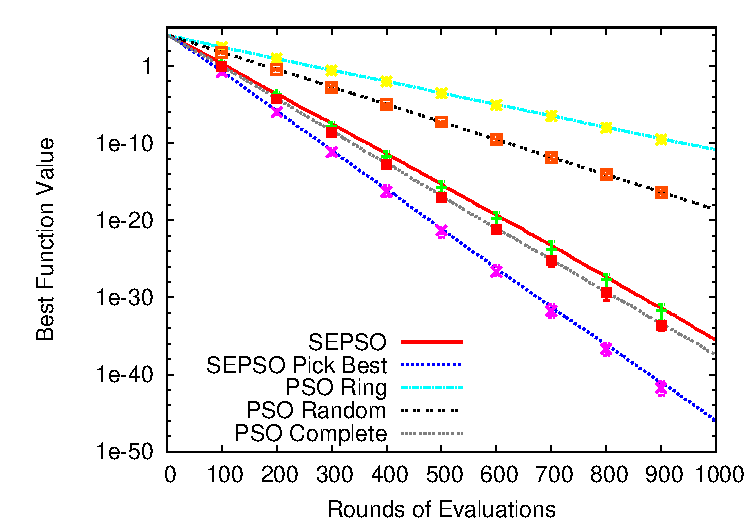
\includegraphics[width=.8\columnwidth]{sphere}
  \caption{Function Sphere with a swarm that uses 240 processors per round of
  evaluations.  Our speculative algorithm has a swarm of 30 particles and does
  two iterations per round, while standard PSO algorithms use 240 processors
  and do one iteration per round.}
  \label{fig:basic-sphere}
\end{figure}

Next we look at the function Griewank, defined by the equation $f(\Vec{x}) =
\frac{1}{4000} \sum_{i=1}^D x_i^2 - \Pi_{i=1}^D \cos\left(\frac{x_i}{\sqrt{i}}
\right) + 1$.  It is generally recommended to use the Ring topology when
optimizing the Griewank function, as Complete is prone to premature convergence
on a local optima.  We show results in \fig{basic-griewank1} for swarms of size
30 and 240 using the Ring topology. One can see in the figure that using
speculative evaluation initially outperforms PSO, but gets stuck in a local
optima and is eventually outperformed.  

\begin{figure}
  \centering
  \includegraphics[width=.8\columnwidth]{griewank1}
  \caption{Function Griewank with a swarm that uses 240 processors per round of
  evaluations.}
  \label{fig:basic-griewank1}
\end{figure}

\fig{basic-griewank1} is slightly deceptive, however, as with Griewank some of
the runs found the global optimum, 0, while some did not.  A more accurate plot
for this function is one showing what percentage of the runs have found the
global optimum at each iteration.  \fig{basic-griewank2} shows such a plot.  A
swarm of size 30 performing the PSO algorithm gets stuck a little less than
half of the time, while 240 particles provides enough exploration to find the
global optimum every time.  As would be expected, when our speculative
algorithm finds the global optimum, it finds it about twice as fast as regular
PSO---it is just performing regular PSO twice as fast with a smaller swarm
size.

\begin{figure}
  \centering
  \includegraphics[width=.8\columnwidth]{griewank2}
  \caption{Function Griewank with a swarm that uses 240 processors per round of
  evaluations.  Instead of showing average function value, we show the
  percentage of runs that have found the global optimum by each iteration.}
  \label{fig:basic-griewank2}
\end{figure}

Because our speculative algorithm got stuck with such a small swarm size, we
ran a set of experiments on Griewank with 800 processors, giving swarms of size
100 and 800 instead of 30 and 240.  \fig{basic-griewank3} shows the results.
\fig{basic-griewank3} is very similar to \fig{basic-griewank2}, except that
speculative evaluation finds the global optimum essentially 100\% of the time.
Thus with a few more processors, our algorithm finds the optimum twice as fast
as the original PSO without a significant loss of accuracy.

\begin{figure}
  \centering
  \includegraphics[width=.8\columnwidth]{griewank3}
  \caption{Function Griewank with a swarm that uses 800 processors per round of
  evaluations.}
  \label{fig:basic-griewank3}
\end{figure}

Lastly we look at a function that does not show any kind of improvement with
this method.  The function Rastrigin is defined as $f(\Vec{x}) = \sum_{i=1}^D
\left(x_i^2 - 10\cos\left(2\pi x_i\right) + 10\right)$.  It has been shown that
with Rastrigin, the more particles there are in the swarm, the lower function
value it finds, up to at least 4000 particles~\cite{mcnabb-cec09}.  Smaller
swarms get caught in local optima.  Because our speculative algorithm has a
significantly smaller swarm size, it gets stuck at higher values while the
larger swarms performing regular PSO continue to improve the best value found.
\fig{rastrigin} shows the results graphically.

\begin{figure}
  \centering
  \includegraphics[width=.8\columnwidth]{rastrigin}
  \caption{Function Rastrigin with a swarm that uses 240 processors per round
  of evaluations.}
  \label{fig:rastrigin}
\end{figure}

\section{Relaxing the Requirements}
\label{sec:relax}

While the idea of speculative evaluation in particle swarm optimization is
intriguing, the results of the previous section show that in many cases it
requires too many extra evaluations to produce competitive results.  On most
functions, the larger swarm size that can be used in regular PSO leads to
better performance than is found by trying to do speculative evaluation.
However, if we keep the idea of speculative evaluation while relaxing the
requirement of exactly reproducing the behavior of the original PSO algorithm,
we see some very impressive results.

We outline three main improvements to speculative evaluation.  First, in
\sec{pickbest} we describe a method that uses all of the information found in
doing speculative evaluations.  Then Sections~\ref{sec:pruning}
through~\ref{sec:wrong} present a technique that reduces the number of
speculative evaluations that need to be done for each particle.  Finally,
\sec{manyiters} shows a method for speculating several iterations ahead,
instead of just one.  \sec{other} presents a few other ideas that seem
promising but need further development.

\subsection{Pick the Best Child}
\label{sec:pickbest}

In performing speculative evaluation as we have described it, $2n+1$
speculative evaluations are done per particle, while all but one of them are
completely ignored.  We can try to make use of those evaluations instead of
throwing them away.  

To use the extra speculative evaluations, instead of choosing the speculative
child that matches that branch that the original PSO would have taken, we take
the child that has the best value.  The methodology is exactly the same as
above except for the process of choosing which speculative child to accept.
The branch that PSO would have taken is ignored, but $\p_t$ must still be
created so it can give the right personal best and neighborhood best values and
positions to $\p_{t+1}$.  The only change needed in \alg{centralized} is in
step 7, where the $\noeval{\s}_{t+1}$ with the best value is chosen from
$\noeval{\sset}_{t+1}$ instead of with the matching branch.

This can be thought of as drawing a number of samples from the next iteration
and accepting the best one.  Speculative particles that move in good directions
are kept.  It seems this modification to PSO would produce more exploitation,
decreasing the amount of exploration.  With functions that are less deceptive
we would expect this method to work well, while performance on more deceptive
functions would probably be hurt.

We show in \fig{sphere-pickbest} the results of using this modification on the
function Sphere.  For ease of labeling, we call the modified algorithm Pick
Best.  As can be seen, where SEPSO did not manage to perform as well as PSO
Complete, Pick Best handily outperforms it with the same number of processors.

\begin{figure}
  \centering
  \includegraphics[width=.8\columnwidth]{sphere2}
  \caption{Function Sphere with a swarm that uses 240 processors per round of
  evaluations, comparing Pick Best with previous results.}
  \label{fig:sphere-pickbest}
\end{figure}

Sphere is a function for which very little exploration needs to be done, so
always keeping the best speculative position found makes intuitive sense.  A
less intuitive result occurs when using Pick Best with the function Griewank.
Griewank is a highly deceptive function prone to premature convergence.  Our
intuition on the behavior of picking the best speculative child is that it
would tend to prematurely converge more often than the original PSO.  However,
as seen in \fig{griewank-pickbest}, Pick Best increases the chance of finding
the optimum while also reducing the number of iterations required to converge.
Perhaps Pick Best encourages local exploitation, while the sparse communication
of the Ring topology still allows for global exploration.

\begin{figure}
  \centering
  \includegraphics[width=.8\columnwidth]{griewank4}
  \caption{Function Sphere with a swarm that uses 240 processors per round of
  evaluations, comparing Pick Best with previous results.}
  \label{fig:griewank-pickbest}
\end{figure}

\subsection{Pruning the Speculative Evaluations}
\label{sec:pruning}

Because the problem facing speculative evaluation is having too many possible
evaluations to perform, a natural step to take is to eliminate some of the
evaluations.  If we could reliably predict which branch were going to be taken,
we could limit ourselves to one speculative evaluation per particle instead of
$2n+1$.  As not all of the branches are evaluated in any given iteration, we
call this technique pruning.  

A naive approach to pruning is to keep track of the last branch taken by each
particle and speculate on that branch.  This turns out to be correct far less
than half of the time on average.

A more principled approach would be to use the statistical behavior of PSO to
find probabilities of taking any particular branch.  While we cannot with
certainty predict which branch a particle will take every time, if we can use
statistics to narrow down the $2(n+1)$ possible evaluations to a few likely
candidates, we can decrease the amount of computation required to do
speculative evaluation and improve our performance.

\subsection{Branch Statistics}

In Table~\ref{tab:evals} we presented all possible branches that a particle
with two neighbors could take.  Here we lump all of the neighbors together and
consider the statistics for the five branches shown in Table~\ref{tab:branches}.

\begin{table}[ht]
  \caption{Five Branches to Consider for Statistics}
  \label{tab:branches}
  \centering
  \begin{tabular}{rc|c}
	&$\pbest$ updated&Source of $\nbest$ update\\
	\hline
	1.&No update&No update\\
	2.&Updated&No update\\
	3.&Updated&The particle itself\\
	4.&No update&Some neighbor\\
	5.&Updated&Some neighbor\\
  \end{tabular}
\end{table}

\begin{table}[ht]
  \caption{Branch Statistics in PSO}
  \label{tab:stats}
  \centering
  \begin{tabular}{c|c|c|c|c|c|c}
	Topology&Function&1&2&3&4&5\\
	\hline
	\hline
	Ring&Sphere&53.0\%&9.3\%&11.4\%&20.2\%&6.2\%\\
	&Griewank&51.7\%&8.4\%&12.2\%&20.7\%&7.0\%\\
	&Rastrigin&49.5\%&4.8\%&14.6\%&21.3\%&9.9\%\\
	&Rosenbrock&51.3\%&7.4\%&12.9\%&21.1\%&7.3\%\\
	\cline{2-7}
	&Average&{51.3\%}&{7.5\%}&{12.8\%}&{20.8\%}&
	{7.6\%}\\
	\hline
	\hline
	Random&Sphere&66.7\%&11.9\%&2.6\%&15.6\%&3.1\%\\
	&Griewank&69.0\%&10.9\%&2.5\%&14.9\%&2.7\%\\
	&Rastrigin&81.9\%&5.5\%&1.5\%&10.0\%&1.0\%\\
	&Rosenbrock&74.2\%&7.7\%&2.2\%&14.0\%&1.8\%\\
	\cline{2-7}
	&Average&{73.0\%}&{9.0\%}&{2.2\%}&{13.6\%}&
	{2.2\%}\\
	\hline
	\hline
	Complete&Sphere&31.9\%&9.2\%&0.2\%&45.1\%&13.5\%\\
	&Griewank&35.3\%&8.4\%&0.2\%&44.1\%&11.9\%\\
	&Rastrigin&47.7\%&6.7\%&0.2\%&38.2\%&7.0\%\\
	&Rosenbrock&35.3\%&3.4\%&0.3\%&54.4\%&6.6\%\\
	\cline{2-7}
	&Average&{37.6\%}&{6.9\%}&{.2\%}&{45.5\%}&
	{9.8\%}\\
	\hline
	\multicolumn{7}{l}{The numbers in the column headings refer to branch
	numbers in Table~\ref{tab:branches}.}
  \end{tabular}
\end{table}

Row 1 in Table~\ref{tab:branches} corresponds to the phenomenon commonly called
stagnation in the literature, but only with a single particle.  As an
interesting aside, we found that complete stagnation practically never occurs
in PSO, though frequently large percentages of the swarm are stagnant.
Iterations where the entire swarm is stagnant average less than 2 in 1000
iterations, unless the swarm converges beyond machine precision.  When graphs
of the best function value flat-line, what really has happened is a contraction
of the particles' velocity, not stagnation in the technical sense.  

We seek to find the probability of taking any given branch, given whatever
information is needed: $\prob(B_t|\cdot)$.  In finding these probabilities, we
do not attempt to derive any distribution from the PSO equations, we simply
look at empirical distributions.  However, even with empirical distributions,
the problem with this approach is that it is not clear what information
influences the probability of taking a branch.  The failure of the naive
approach seems to say that the previous branch, $B_{t+1}$, is not incredibly
useful.  We look at two factors that we believe have a significant influence on
$\prob(B_t)$: topology and function.  Thus we are looking at $\prob(B_t|T,F)$.

We show in Table~\ref{tab:stats} with what percentage a particle takes each of
these branches for three different topologies and four different functions.
All of our statistics are from swarms of 240 particles.  Brief experimentation
showed that other swarm sizes had similar statistics.  We ran 750 iterations on
all combinations of functions and topologies except for the functions Griewank
and Rastrigin with the Complete topology.  We found that those runs frequently
converged past machine precision after 500 iterations, and that led to
erroneously high values for the probability of stagnation.  Instead we ran for
only 450 iterations on those two combinations.  All of our results were
averaged over 20 runs of the algorithm; thus the probabilities presented are
the averages of 3.6 million trials for the branch taken (2.16 million for the
two with only 450 iterations).  Table~\ref{tab:stats} contains the results,
with the branch number coming from Table~\ref{tab:branches}.  We have already
defined the functions Sphere, Griewank, and Rastrigin.  Rosenbrock is defined
as $f(\Vec{x}) = \sum_{i=1}^D \left(100(x_{i+1}-x_i^2)+(x_i-1)^2\right)$.

The probabilities presented in Table~\ref{tab:stats} are interesting in and of
themselves and could probably be used to better understand the characteristics
of various topologies.  It is notable that there is small variation between
functions in any given topology, but the variation across topologies is far
greater.  However, our concern is with speculative evaluation.  We are
interested in predicting the branch that any given particle will take at a
particular iteration.  For our purposes, it appears that given a topology, the
probability of selecting a branch and the function are independent, or
$\prob(B_t|T,F) \approx \prob(B_t|T)$.

From Table~\ref{tab:stats} we can see that with the Random topology, we can
pick the first branch, corresponding to stagnation, and be right around 70\% of
the time.  With the Ring topology, we would be right 50\% of the time.
Branches four and five really correspond to several actual branches, as all of
the neighbors are lumped together.  The 20\% probability of taking branch four
with the Ring topology can be split into two branches, as there are only two
neighbors.  It also turns out that the neighbor that last updated the
neighborhood best is the most likely to update it next time, so keeping track
of that information could be fruitful in trying to predict that branch.

The statistics for the Complete topology are less promising, as there are 240
neighbors that branch four splits into, instead of two.  Pruning does, however,
allow for the possibility of using the Complete topology in speculative
evaluation while avoiding the explosion in the number of evaluations it would
otherwise entail.  Though pruning makes its use possible, we still found the
communication costs in our parallel environment prohibitive, so we do not
present any results for the Complete topology here.

With the other topologies, however, there are a few branches with very high
probabilities, so we can have hope that cutting out some of the evaluations
that have low probability will lead to an increase in overall performance.  In
order to implement this kind of pruning, the only change that needs to be made
to \alg{centralized} is in Step 2, where the speculative children are
generated.  Instead of generating all possible speculative children, generate
the subset of the children that is desired.

\subsection{What if we guessed wrong?}
\label{sec:wrong}

When not all of the branches are evaluated, there is some probability of not
evaluating the branch that was actually taken by the original particle.  We 
need to decide what to do in this case.  

One possibility is to leave the particle as it is, not accepting any of the
speculative evaluations, because none of them were correct.  This leads to
particles being at different iterations, as some particles guess correctly
while others do not.  Thus we lose exact compatibility with the original PSO,
though this particular relaxation is nothing new; asynchronous adaptations of
PSO do the same thing.  As an aside, it is equivalent in this case to simply
increment the iteration number of particles which fail to correctly predict
their branch.  This keeps the iteration number constant across all particles,
simplifying the work needed to be done in determining neighbors when dynamic
topologies are involved.  We call this technique Social Promotion.

Another possibility is to pick the best child, as described in \sec{pickbest}.
This ignores the fact that the branch might have been wrong; we do not care,
because we just want the child that had the best value, anyway.  In almost all
of the experiments that we ran, it turned out that picking the best child
performed better than keeping the particle back an iteration.

There are a large number of ways to prune speculative evaluations.  We
experimented with several, but present results only for one possible pruning.
The pruning we present uses only the two most probable branches in the Random
topology, as seen in~\ref{tab:stats}, the two branches where the $\nbest$ value
was not updated.  Those branches are also convenient in that no messages are
needed from neighbors in order to produce the positions of the speculative
particles---in distributed frameworks using several rounds of communication
(see \sec{distributed}), one of the rounds of communication can be dropped
entirely.

Because we are now only doing two speculative evaluations per particle, with
240 processors we can have a swarm of size 80, instead of the 30 particles in
previous experiments.  

In \fig{sphere-pruned}, we show the results of this simple pruning on the
function Sphere.  As can be seen, the larger number of particles that pruning
allows results in better results when picking the best speculative child.  
When rejecting all speculative children no real improvement is seen.

\begin{figure}
  \centering
  \includegraphics[width=.8\columnwidth]{sphere3}
  \caption{Function Sphere with a swarm that uses 240 processors per round of
  evaluations, comparing pruning with previous results.}
  \label{fig:sphere-pruned}
\end{figure}

When looking at the function Griewank, presented in \fig{griewank-pruned}, we
see different results.  Our intuition about picking the best child is more
correct in this case; while adding 50 more particles to the swarm, Pick Best
with pruning still gets stuck more often than the original Pick Best.  However,
Social Promotion does well in this case, finding the optimum every time and
faster than the original PSO, without the need to increase the number of
processors.

\begin{figure}
  \centering
  \includegraphics[width=.8\columnwidth]{griewank5}
  \caption{Function Griewank with a swarm that uses 240 processors per round of
  evaluations, comparing pruning with previous results.}
  \label{fig:griewank-pruned}
\end{figure}

\subsection{More than one iteration ahead}
\label{sec:manyiters}

We need not simply produce speculative children for the next iteration.  We can
view all possible speculative evaluations for a particle as an infinite tree
with branching factor $2n+1$.  As we have already seen that doing one full
level of the tree produces too many extra evaluations to be profitable, it is
incredibly unlikely that doing two full iterations would produce decent
results.  But, if the idea of speculating more than one iteration ahead is
combined with wisely pruning the possible evaluations based on branch
statistics, we can use just a few extra evaluations to go two or more
iterations ahead on the most likely branches.

When speculating more than one iteration ahead, the idea of picking the child
that matches the correct branch, and holding back the particle if no child
matches the branch, does not make very much sense, as correct branches can only
be determined for the first iteration.  Thus when speculating more than one
iteration ahead we always pick the child that has the highest value.

The question of which branches to take in this infinite tree is an intriguing
one that we can only begin to explore here.  If the branch corresponding to
stagnation has a 75\% chance of being taken, as in the Random topology with
most functions, we could speculate three iterations ahead on that branch and
still have a 42\% chance of predicting correctly.  However, intuition would say
that perhaps it is better to hope that the particle is productive instead of
stagnant, so a branch where the particle updates its personal best might be
more fruitful to try.  In our experiments we try just one of the countless
possibilities, but that one turns out to work extremely well.  More work is
needed to compare the different branching possibilities on various functions.

The combination of branches we tried uses seven speculative evaluations per
particle, matching the swarm size of the original speculative algorithm.  The
seven evaluations we used corresponded to several iterations of branches 1 and
2 in Table~\ref{tab:branches}.  Two of the evaluations were just one iteration
ahead, four were two iterations ahead, and one was three iterations ahead.  The
evaluations that were one iteration ahead were branches 1 and 2; those that
went two iterations ahead were formed by taking either branch 1 or 2 and then
branch 1 or 2; and the evaluation going three iterations ahead followed branch
1 on all three iterations.

The results when optimizing the function Sphere, presented in
\fig{sphere-manyiters}, are rather astounding.  When 240 processors are
available for use, performing speculative evaluation several iterations ahead
finds values an average of 46 orders of magnitude better than using the
processors to perform the standard PSO algorithm with 240 particles.

\begin{figure}
  \centering
  \includegraphics[width=.8\columnwidth]{sphere4}
  \caption{Function Sphere with a swarm that uses 240 processors per round of
  evaluations, comparing speculating several iterations ahead with previous
  results.}
  \label{fig:sphere-manyiters}
\end{figure}

With the function Griewank, the premature convergence problems inherent in
picking the best child are exacerbated when speculating several iterations
ahead.  When the algorithm converges, it converges quicker than any other 
method we tried.  However, it also got stuck and failed to find the optimum
more than any other method.  In order for this method to be consistently useful
on functions like Griewank, it seems that more processors are required.  The
results are shown in \fig{griewank-manyiters}.

\begin{figure}
  \centering
  \includegraphics[width=.8\columnwidth]{griewank6}
  \caption{Function Griewank with a swarm that uses 240 processors per round of
  evaluations, comparing speculating several iterations ahead with previous
  results.}
  \label{fig:griewank-manyiters}
\end{figure}

\subsection{Other possibilities}
\label{sec:other}

One issue remains.  What if we really want a swarm of 50 particles, but we have
230 processors to use?  The methods we have thus far presented do the same
thing for every particle, and thus would require some multiple of 50
processors---we would have 30 extra processors with nothing to do.  It might
very well be the best idea to simply adjust the swarm size slightly, but we
present another method that allows particles to behave differently, some doing
more evaluations than others.

If we use the concept of tokens commonly used in multi-robot stuff (see, for
example, \dots), we can specify a number of tokens available for particles to
use, where each token corresponds to a speculative evaluation.  Whichever
method is used to decide which evaluations to do, they are prioritized so that
particles with only one or two tokens perform the most valuable speculative
evaluations.  Particles that perform well keep their tokens, and particles that
perform poorly send one token (if they have one) to another random particle in
the swarm.

We choose to define ``perform poorly'' as a failure to update the personal best
when the original particle's position is evaluated.  Clearly there are other
possible methods of deciding when to give up tokens, but many of the methods
that sound the best are difficult in distributed environments, like giving
tokens to that particles that most recently found the globally best positions.
The use of a central machine to decide which particles get tokens would help to
facilitate such methods.

There are thus two distinct uses for tokens.  First, they could be used to try
to evenly spread extra evaluations due to an incompatible number of particles
and processors.  In cursory experimentation, we found that this was not a very
effective use of tokens.  In virtually every case we tried, it was better to
simply change the number of particles to match the number of processors, and 
spread the speculative evaluations evenly throughout the swarm.

The other, more compelling reason to use tokens is to intelligently and
dynamically allocate speculative evaluations to particles that are performing
well.  This really only makes sense when speculating several iterations ahead;
after one or two speculative evaluations, the added benefit from also
evaluating the low-probability branches is negligible.  But by intelligently
allocating speculative evaluations, particles that are going in good directions
move faster by speculating farther with extra tokens, while particles that are
not doing as well lose their tokens.  Those particles likely contribute to the
exploration of the algorithm, and when they find good locations, they start
keeping their tokens, switching roles to become productive particles
themselves.  This approach is very similar in concept to other dynamic swarms,
like the TRIBES method proposed by Clerc (cite).

As in the previous section, we can only offer a very preliminary exploration of
the possibilities of using tokens to improve the allocation of speculative
evaluations to particles.  We used a distributed parallel PSO framework, and in
this setting determining which particles are performing the best globally is
difficult without extensive communication.  Thus we only present results for
the one method of token allocation described above.  

The only function for which we saw a benefit when using this technique was
Griewank.  As seen in \fig{griewank-token}, using tokens increased the chance
of finding the optimum to 100\%, while still using far fewer iterations than
standard PSO.  We assume that the relatively poor performance of the technique
on other functions is due to the lack of better token allocation.

\begin{figure}
  \centering
  \includegraphics[width=.8\columnwidth]{griewank7}
  \caption{Function Griewank with a swarm that uses 240 processors per round of
  evaluations, comparing token-based allocation with previous results.}
  \label{fig:griewank-token}
\end{figure}

\section{Conclusions}
\label{sec:conclusion}

We have described a new technique for using processors in parallel PSO to
improve the performance of the algorithm.  To our knowledge, this is the first
time extra processors have been used to do anything in PSO besides increase the
swarm size.  In an increasingly parallel world, such advancements will prove to
be crucial to the continued effectiveness of PSO.

We have detailed how to perform speculative evaluation in PSO in several
different parallel frameworks.  Using this methodology, the behavior of the
original PSO algorithm can either be exactly reproduced, two iterations at a
time, or the behavior can be modified in order to improve performance.  While
exactly reproducing PSO often uses too many extra processors to be useful, when
we allow ourselves some freedom with the algorithm we see great improvements
over previous methods.  We have shown results that conclusively demonstrate the
superiority of our techniques for several functions over naively adding
particles to the swarm when extra processors are available.

Though our methods show great improvements on some functions, they do not work
for all functions.  As is commonly known, in PSO there is a trade-off between
exploration and exploitation.  Some functions need only minimal exploration,
and some never seem to have enough.  Increasing the swarm size is a natural way
to increase exploration in a parallel environment.  However, once ``enough''
exploration has been reached for any particular function, adding additional
particles adds only incremental benefits.  A better use of the additional
processors, as we have shown, is to perform some amount of speculative
evaluation.

Sphere is a function for which only a very small amount of exploration needs to
be done, and our speculative methods show improvements on Sphere of over 40
orders of magnitude.  Such functions are perfect for our methods.

Rastrigin, on the other hand, is a function for which increasing the swarm size
up to 4000 particles still shows improvements in the performance of the
algorithm.  With such functions, the smaller swarm size required by speculative
evaluation is not able to produce enough exploration to perform better than
standard PSO at the swarm sizes we were able to experiment with.

Griewank is a function in between Sphere and Rastrigin.  It is highly deceptive
and is prone to premature convergence, but by adding particles to the swarm a
point is reached where ``enough'' exploration is done, and the algorithm finds
the optimum essentially all of the time.  For such functions, the best approach
seems to be to increase the swarm size until ``enough'' exploration is reached,
then use extra processors to perform speculative evaluation and increase the
number of iterations performed.  Sphere and Rastrigin can be thought of as
special cases of these types of functions; Sphere simply needs a very small
swarm size to produce ``enough'' exploration, and Rastrigin requires a very
large swarm.  We expect that for all functions there is a swarm size for which
additional particles are less useful than additional iterations.

Large parallel clusters are often required to successfully optimize practical
modern problems.  To properly use PSO with such clusters, a balance needs to be
made between using processors to increase the swarm size and using them to
increase the speed of the algorithm.  This work is a first step in that
direction.

\section{Future Work}
\label{sec:future}

This work represents the first attempt of which we are aware at using
additional processors in parallel with PSO to do something other than either
add particles to the swarm or parallelize the evaluation of the objective
function.  We anticipate that many future advancements can be made.

We have speculated that our Pick Best method simply draws a number of samples
from the next iteration of the sampling distribution of PSO and keeps one of
them.  It would then be expected that the sampling distribution of that method
is very similar to the distribution of the original PSO.  This remains to be
proven, or even demonstrated empirically.

We gave a passing glance to some very interesting statistical characteristics
of PSO.  Our motivation was to use the statistics to improve our speculative
algorithm, but it seems there are some nuggets in the numbers that could be
used to improve our understanding of the behavior of PSO in general, and what
role a topology plays.  A potentially very fruitful avenue of future work would
be to further analyze the branch statistics in PSO across many functions and
topologies, categorizing both the topologies and the functions and discovering
what it is that makes certain topologies work well with certain functions.
There are also some particles that seem to drive the swarm and others that are
stagnant almost the entire time.  Such information could be used in a
TRIBES-like fashion to determine which particles should be removed from the
swarm, perhaps starting them close to well-performing particles.

We turned what used to be a very simple algorithm with only one major parameter
to tweak (the topology) into a convoluted mess with countless possibilities for
speculative evaluations.  Perhaps future research will be able to narrow down
the endless possibilities into the few best ones, making the algorithm simple
again.  We have presented some small amount of exploration of the possible
alternatives, but our discussion is by no means exhaustive or conclusive.

We gave only a very little attention to the possibilities of token-based
allocation of speculative evaluations to particles.  We imagine that the
benefits of intelligently and dynamically deciding which particles get extra
evaluations could produce very good results.  Future work could explore the use
of a centralized allocator for extra processors or ideas in the multi-robot
task allocation literature, such as auctions, to better assign processors to
particles for speculative evaluations.  While such methods involve extra
communication, with long-running function evaluations the extra overhead of
intelligently allocating resources would likely be negligible.

We have mentioned that this technique has been previously used to parallelize
simulated annealing.  Any other optimization algorithm that only depends on 
current sampling positions when computing the next position to sample can be
parallelized with this technique.  In particular, genetic algorithms produce
future generations by combining individuals from the current generation.  With
a large population size there would be an unwieldy amount of possible future
individuals, but the potential exists to modify the algorithm to use some kind
of speculative evaluation.  A related but quite distinct technique for reducing
computation in evolutionary algorithms was proposed in~\cite{poli-ai06}.


\appendix[Alternate form of message passing]

Here we describe a method that requires only one round of communication for
each pair of iterations, which happens at step 5 of \alg{centralized}.  Many
more messages are needed, but that is sometimes more desirable than
synchronizing all of the machines three times.

This second method only requires one round of passing information because
information about iterations $t$ and $t+1$ is passed at the same time.  Each
processor reconstructs from the messages it receives all of the information
that it needs about its neighbors.  Messages are passed directly after
evaluating each particle and its children, so all messages are of the form of
$\nonbest{\p}_t$ or $\nonbest{\s}_{t+1}$.  The first iteration needs to be
treated specially, so each particle can produce its initial set of speculative
children---neighbors need only pass their initial position.  This kind of
message passing necessitates the careful use of random seeds, so that when each
processor computes the motion equations for its neighbors it gets the same
results as its neighboring processors.

With the results of evaluating $\noeval{\p}_t$ and $\noeval{\sset}_{t+1}$,
along with all of the required messages from neighboring particles, the goal is
to produce $\p_{t+1}$ and output $\noeval{\p}_{t+2}$ and $\noeval{\sset}_{t+3}$
ready to be evaluated for the next iteration.  We first focus on the messages
needed to produce $\p_{t+1}$.

Upon evaluation, $\noeval{\p}_t$ becomes $\nonbest{\p}_t$, needing only to get
its neighborhood best information from its neighbors.  All of its neighbors,
then, must send it a message, so that from their updated personal best at
iteration $t$ the particle becomes $\p_t$.  The work done with the messages
received thus far is just as in regular PSO, and is graphically depicted in 
\fig{messages1}.

\begin{figure}
  \centering
  \psfrag{pt-n}[C][C]{$\nonbest{\p}_{t}$}
  \psfrag{nt-n}[C][C]{$\nonbest{\nset}_{t}$}
  \psfrag{pt}[C][C]{$\p_{t}$}
  \includegraphics[width=.3\columnwidth]{messages1}
  \caption{The production of $\p_{t}$ from the original particle
  $\nonbest{\p}_{t}$ and the messages $\nonbest{\nset}_{t}$.}
  \label{fig:messages1}
\end{figure}

With $\p_t$ we can select the correct speculative child as described above and
produce $\nonbest{\p}_{t+1}$.  Again we show the use of messages thus far
graphically, in \fig{messages2}.  

\begin{figure}
  \centering
  \psfrag{pt-n}[C][C]{$\nonbest{\p}_{t}$}
  \psfrag{nt-n}[C][C]{$\nonbest{\nset}_{t}$}
  \psfrag{pt}[C][C]{$\p_{t}$}
  \psfrag{pt1-n}[C][C]{$\nonbest{\p}_{t+1}$}
  \psfrag{st1-n}[C][C]{$\nonbest{\sset}_{t+1}$}
  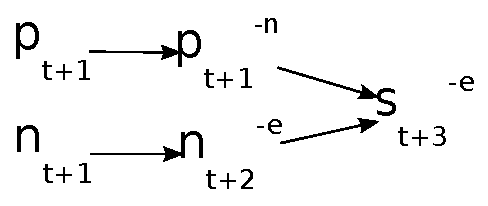
\includegraphics[width=.5\columnwidth]{messages2}
  \caption{The production of $\nonbest{\p}_{t+1}$ from the original particle 
  $\nonbest{\p}_{t}$, messages $\nonbest{\nset}_{t}$ and
  $\nonbest{\sset}_{t+1}$, and intermediate particles.}
  \label{fig:messages2}
\end{figure}

We then need the set of neighbors to $\nonbest{\p}_{t+1}$,
$\nonbest{\nset}_{t+1}$, so we can update $\nonbest{\p}_{t+1}$'s neighborhood
best.  To produce each neighbor $\nonbest{\n}_{t+1}$, we need the same
information for the neighboring particle that we needed to produce the original
particle, $\nonbest{\p}_{t+1}$; we need the original neighbor particle, its
speculative children, and its neighbors.  With that information, the set
$\nonbest{\nset}_{t+1}$ can be obtained by following the same process used to
obtain $\nonbest{\p}_{t+1}$.  We graphically show the messages needed to
produce $\nonbest{\nset}_{t+1}$ in \fig{messages3}.  Note that it looks
identical to \fig{messages2}, just with different sets of particles.

\begin{figure}
  \centering
  \psfrag{nt-n}[C][C]{$\nonbest{\nset}_{t}$}
  \psfrag{nnt-n}[C][C]{$\nonbest{\nnset}_{t}$}
  \psfrag{nt}[C][C]{$\nset_{t}$}
  \psfrag{nt1-n}[C][C]{$\nonbest{\nset}_{t+1}$}
  \psfrag{nst1-n}[C][C]{$\nonbest{\nsset}_{t+1}$}
  \includegraphics[width=.6\columnwidth]{messages3}
  \caption{The production of each $\nonbest{\n}_{t+1}$ from the original
  particle $\nonbest{\n}_{t}$, messages $\nonbest{\nnset}_{t}$ and
  $\nonbest{\nsset}_{t+1}$, and intermediate particles.  $\nnset$ is the set of
  neighbors for each particle $\n$, and $\nsset$ is the set of $\n$'s
  speculative children.  Note the similarity between this and \fig{messages2}.}
  \label{fig:messages3}
\end{figure}

With $\nonbest{\nset}_{t+1}$ and $\nonbest{\p}_{t+1}$, we can produce
$\p_{t+1}$.  This is shown in \fig{messages4}.  Note that we just combined
Figures~\ref{fig:messages2}~and~\ref{fig:messages3}, putting them together
to make $\p_{t+1}$, as all the particle needs is its neighborhood best to be
updated.

\begin{figure}
  \centering
  \psfrag{pt-n}[C][C]{$\nonbest{\p}_{t}$}
  \psfrag{nt-n}[C][C]{$\nonbest{\nset}_{t}$}
  \psfrag{pt}[C][C]{$\p_{t}$}
  \psfrag{pt1-n}[C][C]{$\nonbest{\p}_{t+1}$}
  \psfrag{st1-n}[C][C]{$\nonbest{\sset}_{t+1}$}
  \psfrag{nt-n}[C][C]{$\nonbest{\nset}_{t}$}
  \psfrag{nnt-n}[C][C]{$\nonbest{\nnset}_{t}$}
  \psfrag{nt}[C][C]{$\nset_{t}$}
  \psfrag{nt1-n}[C][C]{$\nonbest{\nset}_{t+1}$}
  \psfrag{nst1-n}[C][C]{$\nonbest{\nsset}_{t+1}$}
  \psfrag{pt1}[C][C]{$\p_{t+1}$}
  \includegraphics[width=.8\columnwidth]{messages4}
  \caption{The production of $\p_{t+1}$ from the original particle 
  $\nonbest{\p}_{t}$, messages $\nonbest{\nset}_{t}$, $\nonbest{\sset}_{t+1}$,
  $\nonbest{\nnset}_{t}$, and $\nonbest{\nsset}_{t+1}$, and intermediate
  particles.  Note that this is just a combination of \fig{messages2} and
  \fig{messages3}.}
  \label{fig:messages4}
\end{figure}

In order to get $\p_{t+1}$, then, a particle needs to receive messages from its
neighbors, its neighbors' neighbors, its speculative children, and its
neighbors' speculative children.  The particle $\p_{t+1}$ can be passed to some
central machine to track the progress of the algorithm, and it can be moved to
$\noeval{\p}_{t+2}$ in order to start the next iteration.

The next goal is to produce the set $\noeval{\sset}_{t+3}$.  As described
above, the necessary components to produce $\noeval{\sset}_{t+3}$ are
$\noeval{\p}_{t+2}$ and the neighbors of $\noeval{\p}_{t+2}$,
$\noeval{\nset}_{t+2}$.  We already have $\noeval{\p}_{t+2}$, so what remains
is to produce $\noeval{\nset}_{t+2}$.  It is sufficient to obtain
$\nset_{t+1}$, as each neighbor particle $\n_{t+1}$ can be moved with the
motion equations to $\noeval{\n}_{t+2}$.

We have already described how to use a set of messages to obtain $\p_{t+1}$.
The process is exactly the same to produce each $\n_{t+1}$, requiring the same
messages, only for the neighbor particles instead of the particle itself.
\fig{messages5} shows graphically how $\noeval{\sset}_{t+3}$ is produced.

\begin{figure}
  \centering
  \psfrag{pt1}[C][C]{$\p_{t+1}$}
  \psfrag{nt1}[C][C]{$\nset_{t+1}$}
  \psfrag{nt2-e}[C][C]{$\noeval{\nset}_{t+2}$}
  \psfrag{pt2-e}[C][C]{$\noeval{\p}_{t+2}$}
  \psfrag{st3-e}[C][C]{$\noeval{\sset}_{t+3}$}
  \includegraphics[width=.5\columnwidth]{messages5}
  \caption{The production of $\noeval{\p}_{t+2}$ and $\noeval{\sset}_{t+3}$
  from $\p_{t+1}$ and $\n_{t+1}$, each of which are produced as in
  \fig{messages4}.}
  \label{fig:messages5}
\end{figure}

Having obtained both $\noeval{\p}_{t+2}$ and $\noeval{\sset}_{t+3}$ from the
messages received, the algorithm then moves to the evaluation phase, and the
process repeats itself.  The particles are evaluated, send their messages, and
produce the next set of particles to be evaluated from the messages received.

To perform the entire process, at each message passing round a particle must
receive messages from its neighbors, its neighbors' neighbors, its neighbors'
neighbors' neighbors, its speculative children, its neighbors' speculative
children, and its neighbors' neighbors' speculative children.  With the Ring
topology, that looks like more messages than it really is, as many of the
neighbors' neighbors are duplicates.  With the Random topology, however, the
list of necessary messages could be rather large.  

One more issue arises when dealing with dynamic topologies.  With neighbors
changing each iteration, messages that processors pass to their neighbors need
to be sent to the correct neighbors for each iteration.  In centralized
algorithms and in distributed algorithms with several rounds of message passing
(the first method described above), nothing needs to be changed.  However, in
the case where processors reconstruct information about neighboring particles
from messages, those messages need to be sent to the correct neighbors.  A
particle cannot simply send messages to its neighbors' neighbors'
neighbors---it needs to send messages to its iteration $t$ neighbors' iteration
$t+1$ neighbors, and so on.  For every neighbor outward information is sent,
the iteration also needs to be incremented, as information about neighbors'
neighbors is used during iteration $t+1$, and information about neighbors'
neighbors' neighbors is used to reconstruct information about iteration $t+2$.
Also, this method of message passing again requires the use of random seeds if
the topology is random, so that each processor computes the same neighbors for
a particle as all other processors.

This may seem like an inordinate amount of work, and with some distributed PSO
frameworks it is.  However, other parallel frameworks necessitate this type of
message passing, so we have described how speculative evaluation can be
performed in those circumstances.


\bibliographystyle{unsrt}
\bibliography{%
\bib{wolpert-tec97},%
\bib{merris-01},%
\bib{pso/clerc-tec02},%
\bib{pso/kennedy-icnn95},%
\bib{pso/bratton-sis07},%
\bib{pso/largeswarms/perez-emc05},%
\bib{pso/largeswarms/montes-gecco08.bib},%
\bib{pso/topology/liang-sis05.bib},%
\bib{pso/parallel/belal-ijicis04},%
\bib{pso/parallel/chu-sci06},%
\bib{pso/parallel/jin-aps05},%
\bib{pso/parallel/koh-ijnme06},%
\bib{pso/parallel/mostaghim-report06},%
\bib{pso/parallel/parsopoulos-aia04},%
\bib{pso/parallel/schutte-ijnme04},%
\bib{pso/parallel/venter-wcsmo05},%
\bib{ga/poli-ai06},%
\bib{sim-anneal/parallel/witte-tpds91.bib},%
\bib{pso/topology/kennedy-cec02.bib},%
\bib{pso/topology/mohais-cec04.bib},%
\bib{pso/topology/jordan-gecco08.bib},%
\bib{pso/topology/clerc-oep03.bib},%
\bib{pso/topology/miranda-ijcir08.bib},%
\bib{pso/topology/mendes-phd04.bib},%
\bib{aml/mcnabb-cec07},%
\bib{aml/mcnabb-cec09}}

\end{document}
